% 4. Konzept (Kontext, Ablauf, Anforderungen [Interviews], Konzept [Architektur])
\chapter{Conceptual Design}
\label{chap:conceptual-design}
%This chapter will detail the process of conceptualizing the design of the modular proxy application based on the results of the preceding chapter. First, the requirements are analysed for their potential design implications in section \ref{sec:req-design-implications}. Afterwards the user interactions and domain entities identified in chapter \ref{chap:understanding-the-problem-space} are examined and broken down into communication flows between actors and systems in section \ref{sec:user-interactions-designing-workflow} and individual software components that complete the design are discussed in section \ref{sec:inferring-software-components}. Lastly, an overview of the complete design concept is given in section \ref{sec:abstract-design-concept}, discussing potential advantages and constraints. %TODO: Rewrite & update

%\section{Inferring Software Components}
%\label{sec:inferring-software-components}
Building on the software design of the first prototype presented in section \ref{sec:prototype-design} and the insights gained in section \ref{sec:prototype-insights}, two design concepts were worked out. The following sections will detail components and principles of both concepts.

\section{Design \#1: Singular Proxy Application}
This design concept is based on the general ideas presented in section \ref{sec:prototype-design} (e.g. state-machines, network stacks and pipes) and employs a basic architecture shown in figure \ref{fig:component-view-1}.\\
\begin{figure}[h]
    \centering
    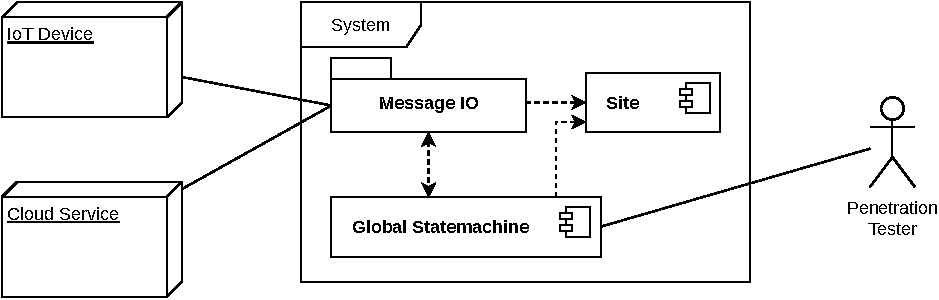
\includegraphics[width=12cm]{img/ch05/component-view-1.pdf}
    \captionof{figure}{High-level component diagram of the proxy application concept}
    \label{fig:component-view-1}
\end{figure}
As discussed in the previous chapter, the requirement \enquote{F2 Network Stacks} introduces the need for dynamically initialized objects which in this concept is implemented by making use of the factory pattern in the \enquote{Site} component. This component allows for registering \emph{Factories} that are used to initialize objects. Similar to the implementation in the first prototype, factories initialize objects using metadata supplied from a configuration file.\\
Communication with other systems is encapsulated into the \enquote{Message IO}-package shown in figure \ref{fig:component-view-2}. Applications that are tested by penetration testers are connected to sockets provided by the \enquote{Gateway} component and temporarily stored in a message queue to be processed by the network stacks organized by the \enquote{Global Statemachine}. Similar to the \enquote{Server} interface used in the first prototype, gateways provide means of communicating with external systems and receiving and sending messages. They are highly abstract and meant to be used for implementing interfaces for any kind of communication protocols and technologies, such as \ac{IP}-based \ac{TCP} and \ac{UDP} communication but also other protocols such as USB, Bluetooth, ZigBee or KNX.
\begin{figure}[h]
    \centering
    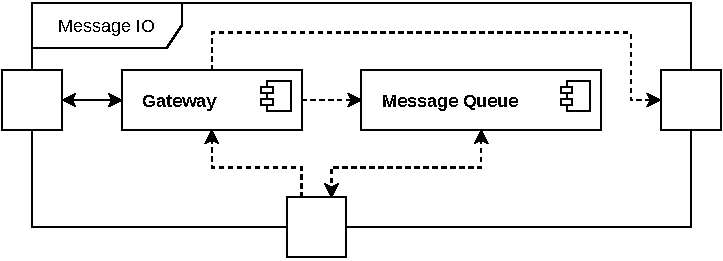
\includegraphics[width=12cm]{img/ch05/component-view-2-messageio.pdf}
    \captionof{figure}{The \enquote{Message IO}-package}
    \label{fig:component-view-2}
\end{figure}
It should be noted that the static view of the design is rather simple due to its dynamic runtime behaviour: many instances and relationships are only instantiated at runtime and not pre-determined. An schematic representation of the dynamic structure and interweaving of state-machines, network stacks and pipes (in this concept called a \enquote{pipeline}) is shown in figure \ref{fig:pipeline}. This figure highlights a series of active state-machines and network stacks which together constitute the active pipeline. \\
Figure \ref{fig:app-activity-fsms} illustrates the recursive nature of this concept processing (dequeued) messages:
\begin{enumerate}
    \item A state-machine $F$ (initialized with the global state-machine instance) relays messages $M$ through its active state $S$'s network stack instance $N$.
    \item In $N$, all of its pipes $P$ process $M$ until the end of $N$ is reached ($P$ does not hold a reference to a succeeding pipe instance). If $F$ holds a reference to a succeeding \ac{FSM}, $F$ is set to this reference and the processes continues from step $1$.
    \item If $N$ does not hold a reference to a nested \ac{FSM}, the end of the network stack is reached and the direction of traversing the network stack is reversed.
    \item $P$ is set to $N$'s last pipe instance and $M$ is processed by $P$ until the start of $N$ is reached (i.e. $P$ does not hold a reference to a preceding pipe instance). If $F$ holds a reference to a preceding \ac{FSM} instance, $F$ is set to this reference, $N$ is set to $F$'s network stack reference and the process continues from step $4$.
    \item If $N$ does not hold a reference to a preceding \ac{FSM}, the beginning of the whole pipeline is reached and $F$ is the global state-machine.
\end{enumerate}

\begin{figure}[h]
    \centering
    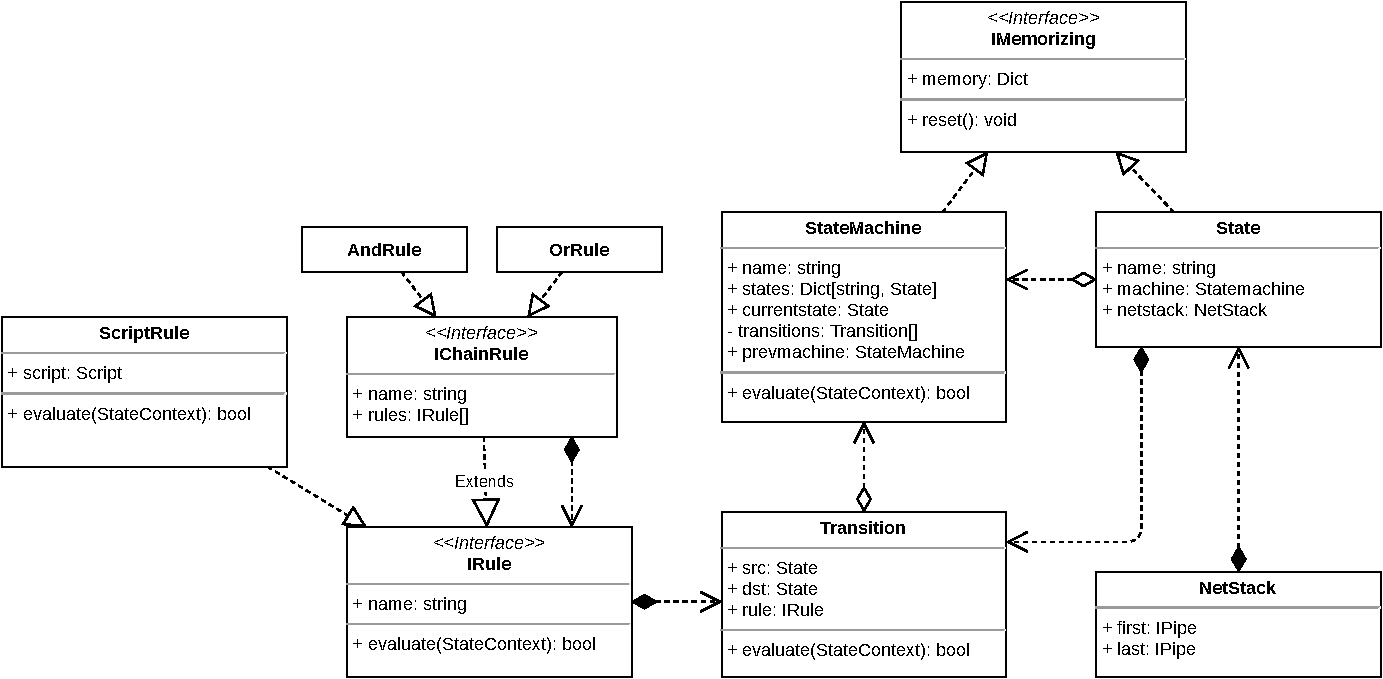
\includegraphics[width=14cm]{img/ch05/classes-1-fsm-rules-netstack.pdf}
    \captionof{figure}{?} %TODO: Describe
    \label{fig:classes-1-fsm-rules-netstack}
\end{figure}
\paragraph{State-Machines} The classes related to the state-machine component are shown in figure \ref{fig:classes-1-fsm-rules-netstack}: \emph{StateMachines} hold a set of \emph{States} and \emph{Transitions}. In order to change states, state-machines evaluate a context by checking each of their transitions for whether their conditions for transition are met or not. This context is an aggregation of the \emph{memory} of each state-machine and their active states in the active pipeline. Transitions are defined by a source state, destination state and an \emph{IRule} that evaluates a given context. Rules can be concatenated with logical $AND$ or $OR$ operators and are designed to be scripts that operate on the given context. This allows the creation of nested rules such as the following one:
\begin{align*}
    \mathbf{changeToWS}(c) & = \mathbf{AND}(\mathbf{clientUpgrade}(c), \mathbf{serverUpgrade}(c))
\end{align*}
In this example, a transition with the above rule would evaluate to $true$ and trigger a state transition in a state-machine when the aggregated memory $c$ of all state-machines and their active states of the active pipeline indicated that an \ac{HTTP} request was detected that requested an upgrade to the \ac{WS} protocol (for instance, $clientUpgrade$ would look for an entry $clientUpgradeRequested$ in $c$ and evaluate its contents) and that an \ac{HTTP} response was detected that confirmed the upgrade request. This would allow a state-machine to detect upgrades of \ac{HTTP} communication to the \ac{WS} protocol.\\
States hold a \emph{NetStack} which in turn encapsulate a series of connected pipes, holding references to this series' first and last elements.
\begin{figure}[h]
    \centering
    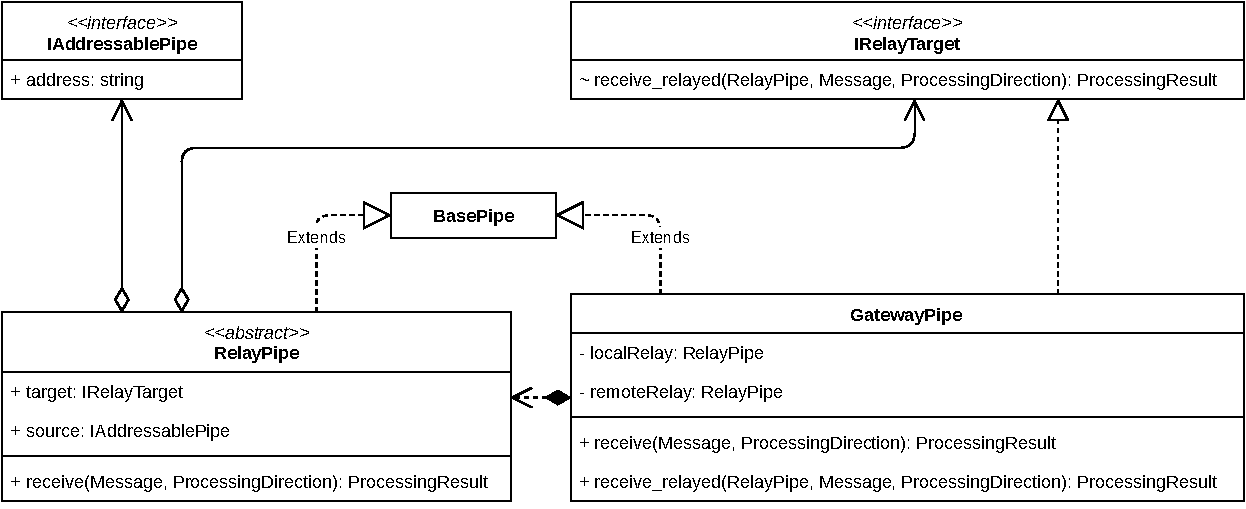
\includegraphics[width=14cm]{img/ch05/classes-3-gateway.pdf}
    \captionof{figure}{?} %TODO: Describe
    \label{fig:classes-3-gateway}
\end{figure}
\paragraph{Gateway} The gateway component is implemented as the \enquote{GatewayPipe} (shown in figure \ref{fig:classes-3-gateway}). Improving on the first prototype's design, the GatewayPipe acts as a multiplexing pipe that accepts messages originating from two \enquote{RelayPipes} that act as two communication ports (e.g. the client device and the cloud server of scenario \#2 described in section \ref{sec:example-scenarios}) that hold information about the address of their communication peers in their address field (e.g. an \ac{IP} address of the remote peer). For instance, two \ac{TCP} client sockets can be handled by two \enquote{TcpPipes} (that inherit from the RelayPipe class), allowing \ac{TCP} packets to be routed into the pipeline via a GatewayPipe.
\paragraph{Pipes} Building upon the approach of routing and processing messages via pipes discussed in section \ref{sec:prototype-design}, this design concept addresses some inconsistencies of the former design and adds needed flexibility. As shown in figure \ref{fig:app-classes-2-pipes}, the \enquote{IPipe} interface persisted and is extended by the \enquote{ITrackablePipe} interface that adds a unique identifier to pipes. This enables the application to easily locate pipes by looking up their identifiers in the \enquote{PipeDirectory}, allowing to interact with and inject messages into individual pipes directly. A \enquote{BasePipe} implements the ITrackablePipe interface as well as simple routing logic for forwarding messages up and down pipelines. However, only \enquote{ProcessingPipes} actually perform any kind of operations on messages directly: they can employ \enquote{IEncoders} for (de-)serialization and \enquote{IProcessors} for transformation of messages. Contrary to the design concept of the first prototype, IEncoders need to specify which data formats they support as source and target encodings. This allows the implementation of multiple IEncoders for the same protocol that work with different source or target data formats. For example, some IEncoder may only provide decoding functionality for raw binary data into \ac{HTTP} messages with raw binary bodies while another implementation provides functionality to encode strings into \ac{HTTP} message bodies. In the first prototype's design, the very concept of filters was only vaguely described and lacked a clear and concise interface. This issue is resolved in this next iteration of the design concept:
\begin{itemize}
    \item Filters are renamed to \enquote{IProcessors} (conveying the purpose and meaning of the interface in its name)
    \item IProcessors specify a \enquote{ProcessingDirection} that determines whether messages shall be processed on their way \emph{down} or \emph{up} a pipeline or in any direction, effectively allowing over transformations on messages. This can be helpful when transformations shall only be applied in one direction or maybe even once in a pipeline, like replacing the value of the \emph{Host} header of a \ac{HTTP} message.
    \item An IProcessor can apply logic to messages in its \emph{process} method that also receives the pipeline's context. The returned \enquote{ProcessingResult} indicates success or failure of the operation or whether the IProcessor directs dropping a message or sending it back up the pipeline.
\end{itemize}
While there are many opportunities for specific implementations of the IProcessor interface, one general implementation is envisioned by the design concept: a simple \enquote{ScriptProcessor} allows penetration testers to supply scripts that are executed at runtime and allow transformation of messages. This directly fulfils the requirement \enquote{"F5 Scripting"}.
\begin{figure}[h]
    \centering
    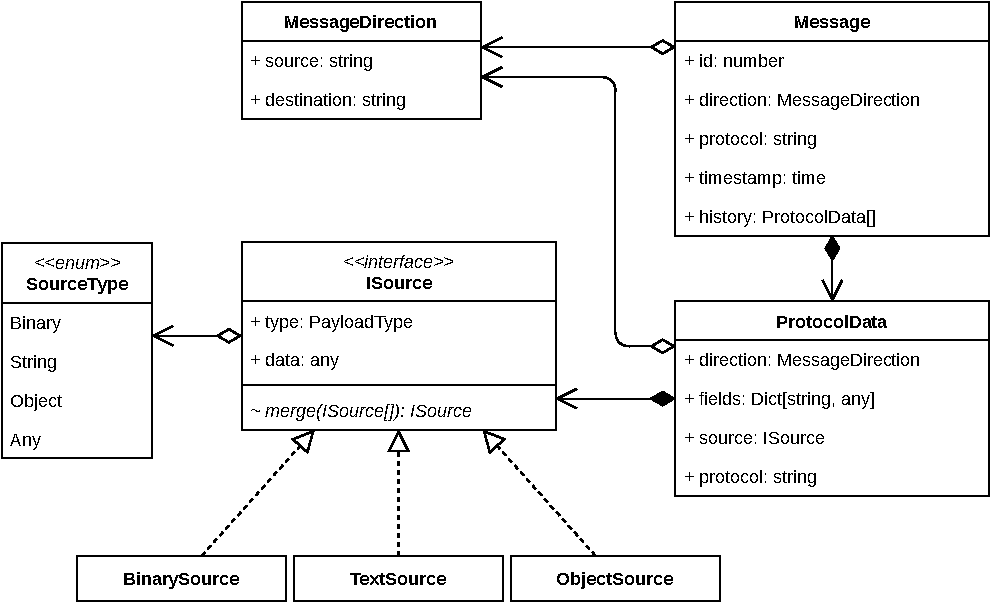
\includegraphics[width=14cm]{img/ch05/classes-4-messages.pdf}
    \captionof{figure}{?} %TODO: Describe
    \label{fig:classes-4-messages}
\end{figure}
\paragraph{Messages}



\section{Design \#2: Distributed Proxy Application}

%\paragraph{Software Architecture} The system employs a server-client architecture that allows to

\emph{TBD} %TODO
\begin{itemize}
    \item \emph{Stream-based: treat communication as streams. message-based systems are simpler and supported by design}
    \item \emph{Server-client: proxy is server, client can interface to control + monitor, communication via REST + WS}
    \item \emph{State-machine: active network stack/pipeline dependent on state of the connection}
    \item \emph{NetStacks: series of pipelines, bound to states}
    \item \emph{Pipes: basic pipes, loose routing, injectable, specialized, generic processors + specialized encoders}
    \item \emph{Factory: parse state-machine and netstack configuration and instantiate + configure instances}
\end{itemize}